\section{Results}




In our study, we conducted extensive experiments to optimize the performance of our mushroom classification model by varying different hyperparameters. Initially, we utilized a learning rate of 0.0001 with the Adam optimizer, which demonstrated promising progress in learning. Both validation and training losses exhibited favorable trends, with the validation loss decreasing while the training loss remained below 90\%, indicating effective learning without significant overfitting. Despite these promising signs, the model's performance did not reach optimal levels.

\begin{figure*}[!ht]
    \centering
    \begin{subfigure}{0.45\textwidth} % Adjust the width as needed
        \centering
        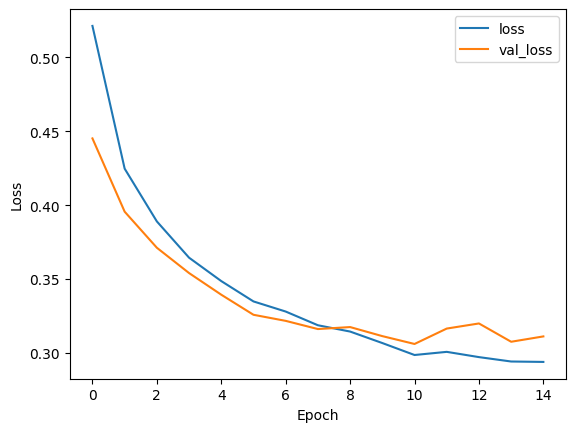
\includegraphics[height=6cm, width=\linewidth]{images/1.loss.png}
        \caption{Training loss vs validation loss} % Add caption for the first figure
    \end{subfigure}
    \hfill
    \begin{subfigure}{0.45\textwidth} % Adjust the width as needed
        \centering
        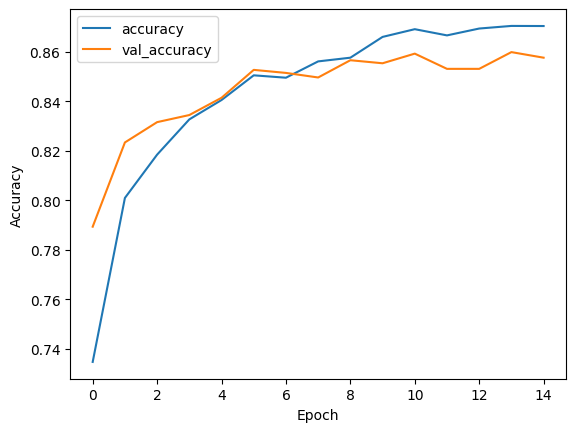
\includegraphics[height=6cm, width=\linewidth]{images/1.Accuracy.png}
        \caption{Training accuracy vs validation accuracy} % Add caption for the second figure
    \end{subfigure}
    \caption{Experiment 1 Metrics: Comparison of loss and accuracy} % Add a general caption for both figures
\end{figure*}



Subsequently, we pursued further refinement by decreasing the learning rate to 0.00002, allowing the model more flexibility to explore smaller steps in the parameter space. Experimenting with different dropout rates and batch sizes, we identified a configuration with a dropout rate of 0.7 and a batch size of 64, which yielded the best results within our hyperparameter search. However, this configuration still resulted in misclassifying 303 poisonous mushrooms as edible and 309 edible mushrooms as poisonous.

\begin{figure}[h]
    \centering
    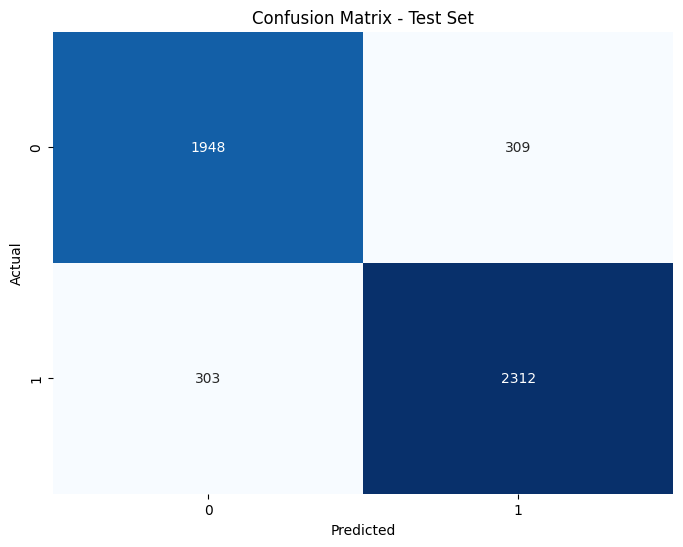
\includegraphics[height=4cm, width=9cm]{images/2.cm.png}
    \caption{Experiment 2 Metrics: Confusion matrix}
\end{figure}


To fine-tune the model further, we adopted an Adam optimizer with a learning rate of 0.001 and increased the dropout rate to 0.8 while maintaining a batch size of 64. This adjustment led to a substantial improvement, reducing misclassifications to 283 edible and 246 poisonous mushrooms. This configuration emerged as the best model in terms of overall accuracy.

\begin{figure*}[!ht]
    \centering
    \begin{subfigure}{0.45\textwidth} % Adjust the width as needed
        \centering
        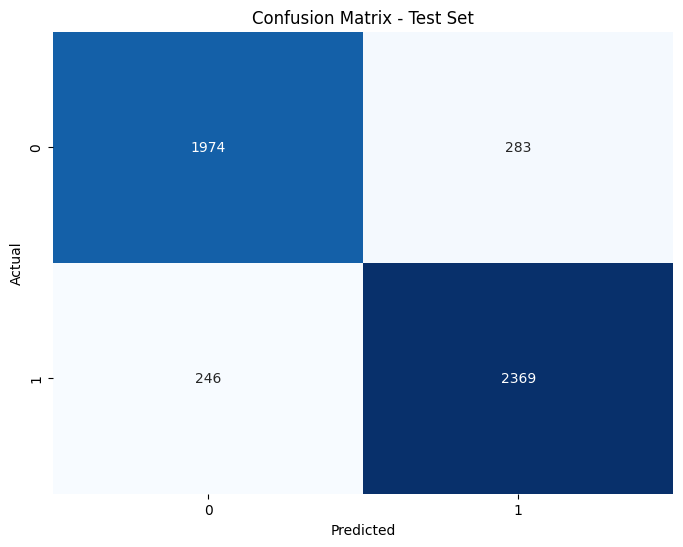
\includegraphics[height=6cm, width=\linewidth]{images/3.cm.png}
        \caption{Confusion matrix} % Add caption for the first figure
    \end{subfigure}
    \hfill
    \begin{subfigure}{0.45\textwidth} % Adjust the width as needed
        \centering
        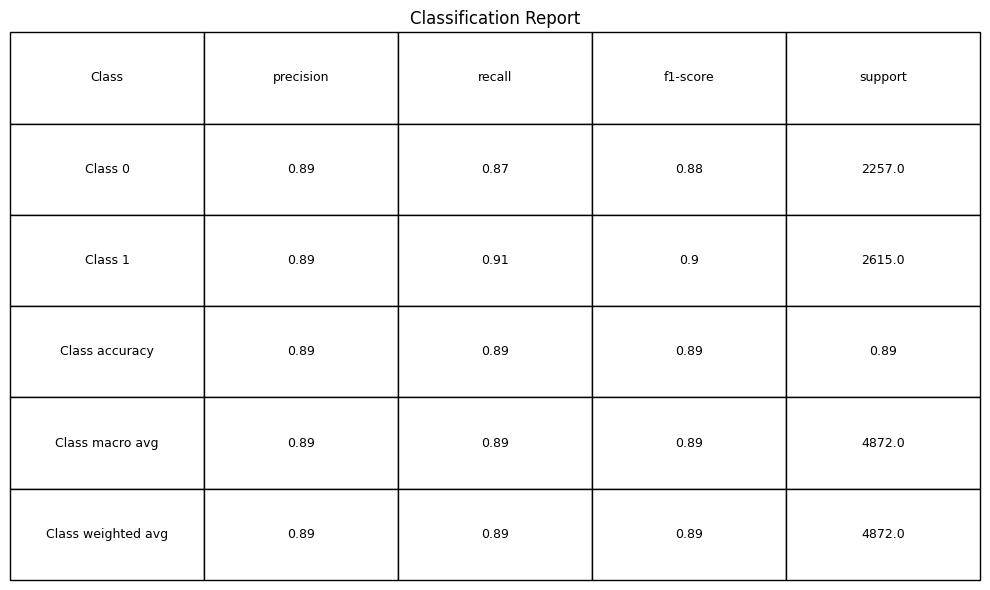
\includegraphics[height=6cm, width=\linewidth]{images/3.cr.png}
        \caption{Classification report} % Add caption for the second figure
    \end{subfigure}
    \caption{Experiment 3 Metrics: Best model for accuracy} % Add a general caption for both figures
\end{figure*}


However, our primary concern was to develop a model capable of correctly classifying poisonous mushrooms, prioritizing the avoidance of misclassifying them as edible. Further exploration led us to a final model configuration with a dropout rate of 0.8, Adam optimizer with a learning rate of 0.001, and a reduced batch size of 48. This model exhibited remarkable performance, misclassifying only 200 poisonous mushrooms as edible, the lowest among all tested models.
\begin{figure*}[!ht]
    \centering
    \begin{subfigure}{0.45\textwidth} % Adjust the width as needed
        \centering
        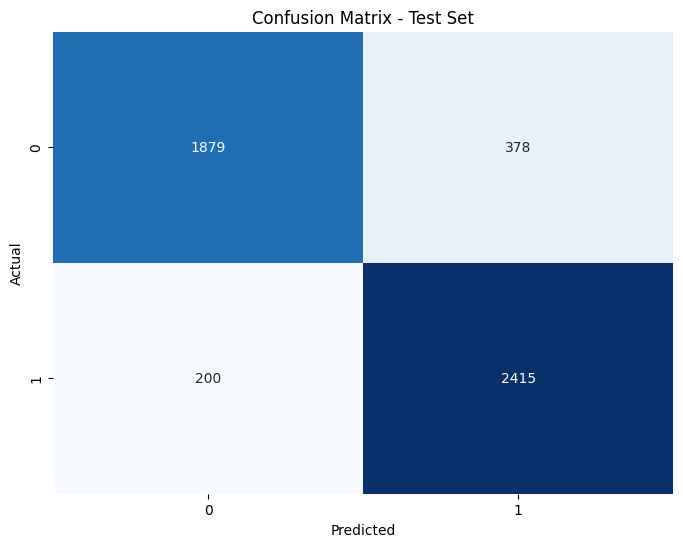
\includegraphics[height=6cm, width=\linewidth]{images/4.cm.png}
        \caption{Confusion matrix} % Add caption for the first figure
    \end{subfigure}
    \hfill
    \begin{subfigure}{0.45\textwidth} % Adjust the width as needed
        \centering
        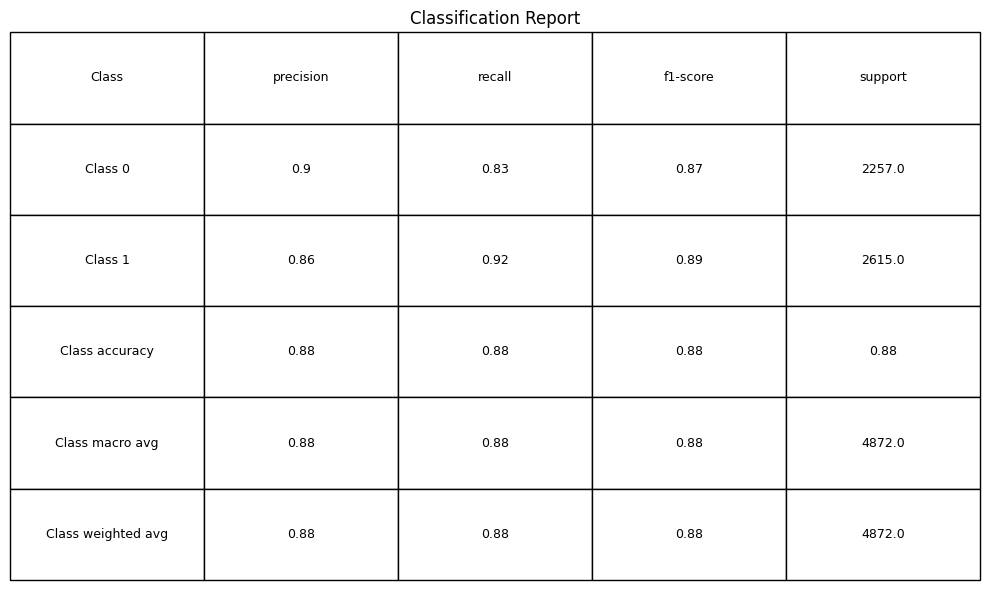
\includegraphics[height=6cm, width=\linewidth]{images/4.cr.png}
        \caption{Classification report} % Add caption for the second figure
    \end{subfigure}
    \caption{Experiment 4 Metrics: Best model to find poisonous} % Add a general caption for both figures
\end{figure*}


The area under the Receiver Operating Characteristic (ROC) curve, often abbreviated as AUC-ROC, is a measure of the model's ability to discriminate between positive and negative classes across all possible classification thresholds. In our case, an AUC-ROC value of 0.96 indicates that our mushroom classification model performs exceptionally well in distinguishing between poisonous and edible mushrooms.

To elaborate, the ROC curve plots the true positive rate (sensitivity) against the false positive rate (1 - specificity) for different threshold values. As the threshold varies, the true positive rate and false positive rate change accordingly, resulting in a curve that represents the trade-off between sensitivity and specificity.

\begin{figure}[!ht]
    \centering
    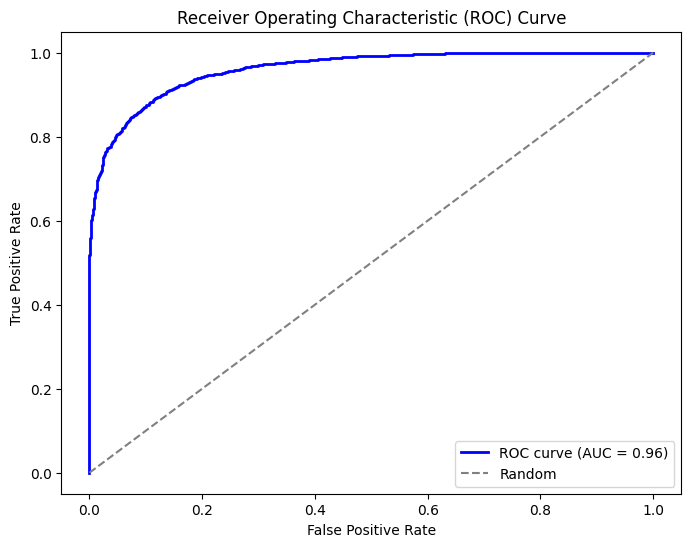
\includegraphics[height=6cm, width=9cm]{images/4.roc.png}
    \caption{Experiment 4 Metrics: ROC curve}
\end{figure}





Moreover, our research contextualized the challenges posed by our dataset, which encompassed a wide range of mushroom species with diverse colors, shapes, and characteristics. Unlike previous studies that often relied on augmented datasets with limited variability, our dataset presented a more formidable task, yet our model, leveraging state-of-the-art EfficientNetB0 architecture and transfer learning, achieved impressive classification accuracy.

Our study underscores the potential of transfer learning and advanced neural network architectures in classifying mushrooms into edible and poisonous categories. Furthermore, it highlights the broader applicability of such models in the classification of other toxic vegetation and fruits, potentially serving as a valuable tool for survival guides during outdoor activities like trekking, hiking, or exploration.

\subsection{Comparing our model with previous model with very high accuracy}
In addition to evaluating our mushroom classification model on our dataset, we also assessed its performance on another dataset containing only three species of edible mushrooms and two species of poisonous mushrooms. A previous study reported an accuracy of 98.5\% and a recall of 98.79\% on this dataset, achieved by dividing it into a 90:10 ratio for training and testing. However, this approach, while yielding high accuracy and recall, may lead to model overfitting due to the presence of similar-looking and augmented images in both training and testing sets.

\begin{figure}[!ht]
    \centering
    \begin{subfigure}{0.45\textwidth}
        \centering
        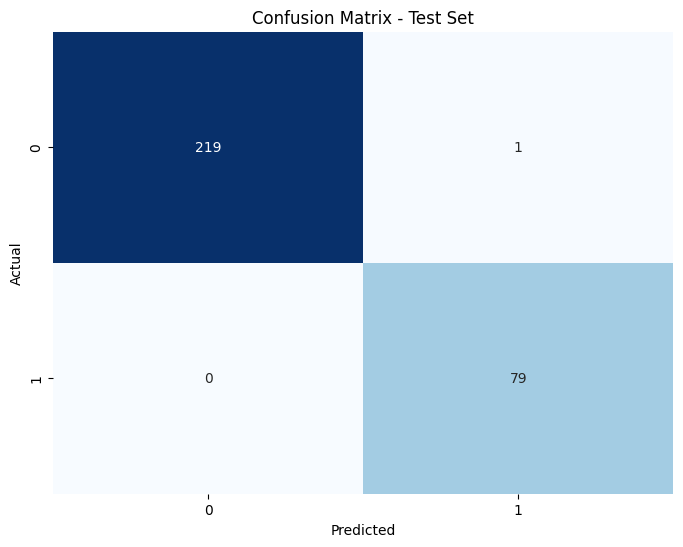
\includegraphics[width=\linewidth]{images/thai.cm.png}
        \caption{Confusion matrix for Thailand dataset}
    \end{subfigure}
    \hfill
    \begin{subfigure}{0.45\textwidth}
        \centering
        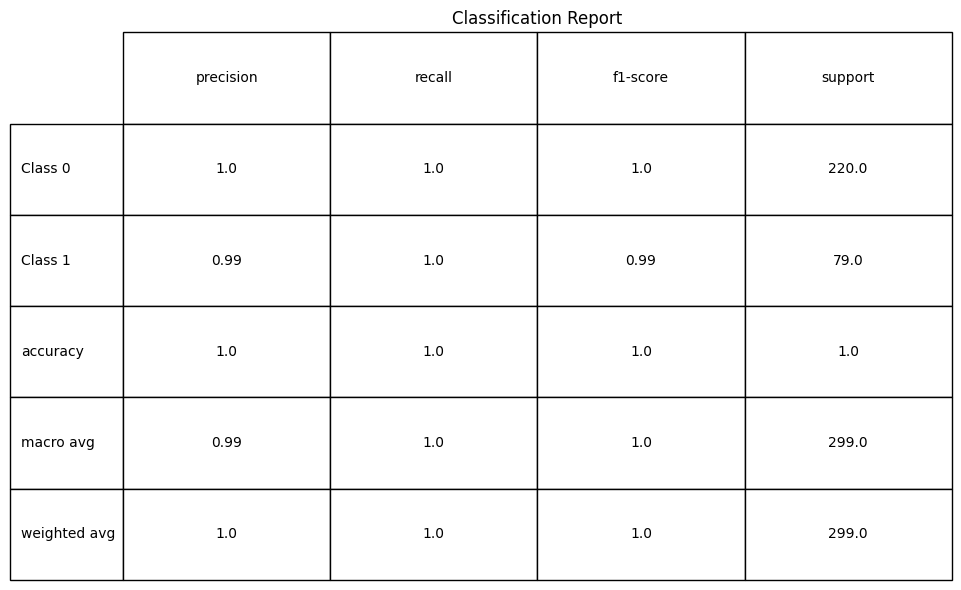
\includegraphics[width=\linewidth]{images/thai.cr.png}
        \caption{Classification report for Thailand dataset}
    \end{subfigure}
    
    \vspace{0.5cm} % Adjust vertical space between rows
    
    \begin{subfigure}{0.45\textwidth}
        \centering
        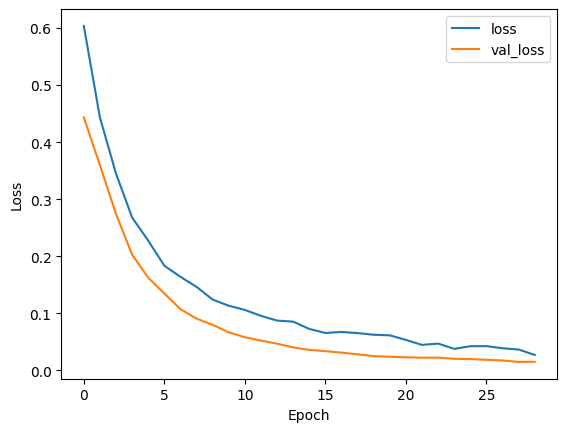
\includegraphics[width=\linewidth]{images/thai.loss.png}
        \caption{Loss curve for Thailand dataset}
    \end{subfigure}
    \hfill
    \begin{subfigure}{0.45\textwidth}
        \centering
        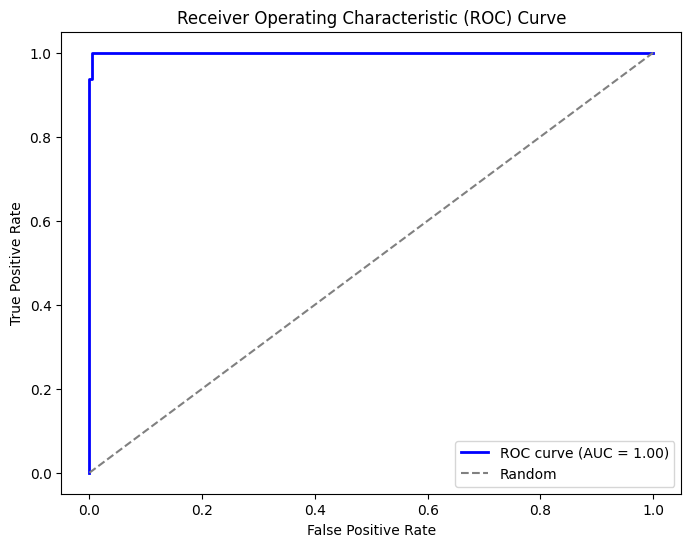
\includegraphics[width=\linewidth]{images/thai.roc.png}
        \caption{ROC curve for Thailand dataset}
    \end{subfigure}
    
    \caption{Plots for Thailand dataset}
\end{figure}

To address this concern, we adjusted the data division by allocating 70\% for training, 15\% for validation accuracy checking, and 15\% for the test set. Remarkably, our model achieved an accuracy of 99.60\% with a recall of 100\%, successfully classifying all poisonous images as poisonous. In contrast, the previous study misclassified two poisonous images as edible, highlighting the potential consequences of using models trained on imbalanced or inadequately validated datasets in real-life scenarios.
